\begin{figure}[h]
 \centering
 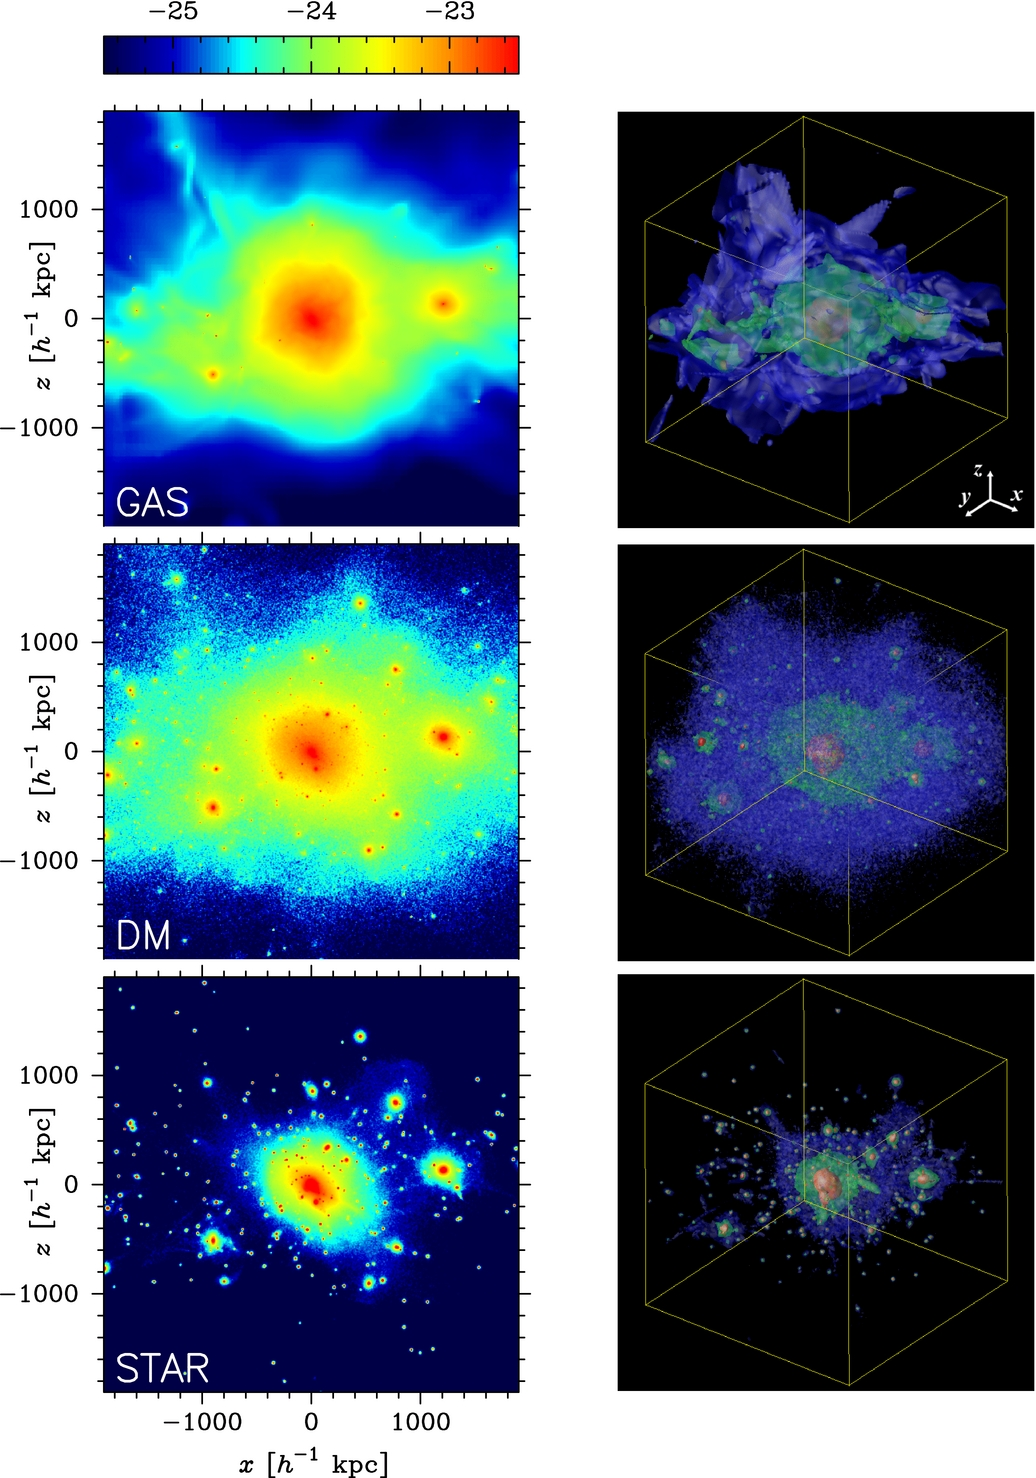
\includegraphics[width=0.6\textwidth]{images/Chapter2/apj464555f1_hr.jpg}
 \caption{Simulation of a galaxy cluster. The first row shows the gas density, the second shows the dark matter density and the last shows the star distribution. The right column shows a 3D rendering of the cluster while the left column shows a projection on the x-z plane.  \citep{Suto_2013}}
 \label{fig:cluster_sim_dm}
\end{figure}

Prior to discussing methods for estimating the masses of galaxy clusters, I'd like to point out the significance of understanding these masses in the first place.

In 1933 Fritz Zwicky was the first one who brought up, that the mass of visible matter of galaxy clusters would be way too small to explain the high movement speeds of the individual galaxies of more than $1000 \, km\cdot s^{-1}$. He estimates, that the cluster mass would have to be 400 times higher as approximated to explain this discrepancy. \citep{Zwicky_1933} To solve this issue, he proposed that the majority of the cluster mass is made out of dark matter causing the observed speeds. Although disputed at first, Zwicky's assumptions are now the basis for dark matter astronomy making galaxy clusters the most important laboratories in the cosmos. To understand the nature of dark matter, it is of key importance to know the cluster masses. Only with precise values, galaxy cluster dynamics such as merges can be accurately observed. More recent simulations of the cluster's dark matter halo show, that the gas distribution is very similar to the distribution of dark matter as seen in \autoref{fig:cluster_sim_dm}. As discussed in \cref{x-ray}, X-ray light is directly being emitted by the hot cluster gas. For this reason, X-ray satellites such as CHANDRA and eROSITA are the best observatories for understanding the distribution of dark matter in galaxy clusters.


